
\lecture{13}{Engines and Refrigerators}{Qiang Zhu}{scribe-name1,2,3}

\section{Heat Engines and Refrigerators}
A heat engine is any device that absorbs heat and converts part of that energy into work. Unfortunately, only part of the energy absorbed as heat can be converted to work. The reason is that the heat, as it flows in, brings along entropy, which must somehow be disposed as waste. 

\begin{figure}[ht]
\centering
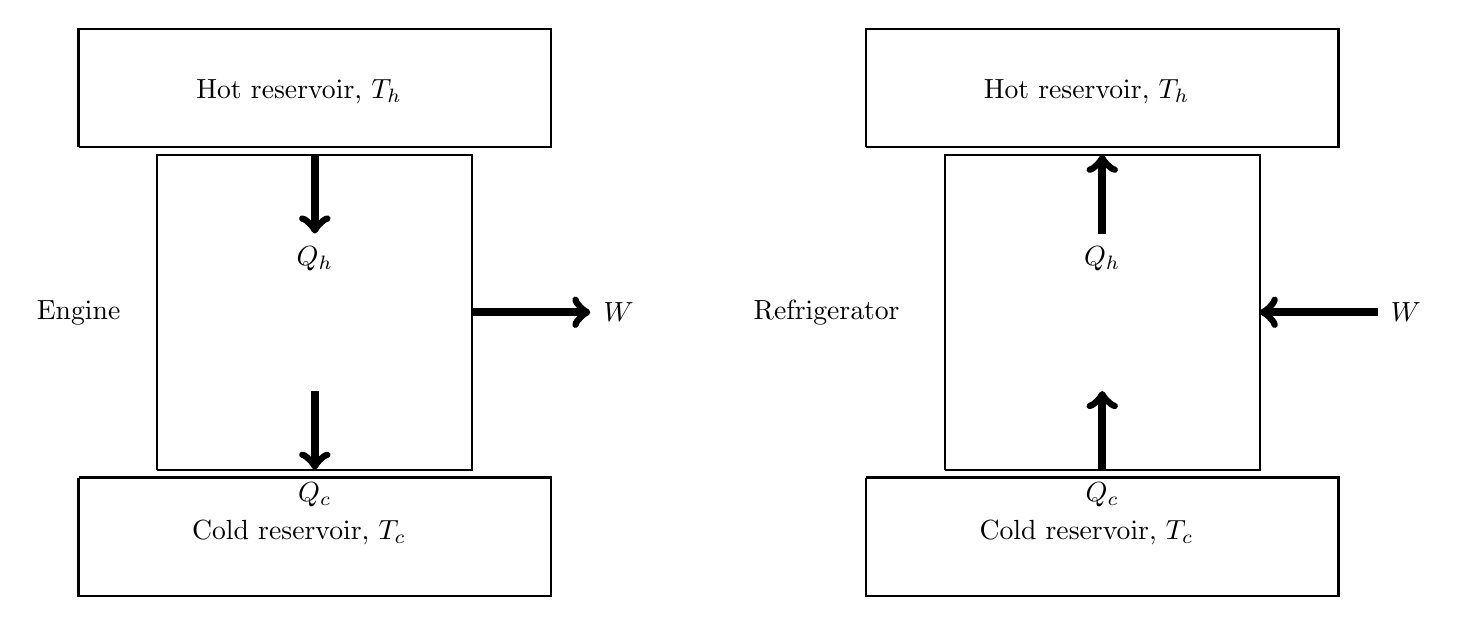
\begin{tikzpicture}[thick]
\draw (0, -2.0) -- ( 0, 2.0) -- (4, 2.0) -- (4,-2.0) -- (0,-2.0);
\draw (-1, 2.1) -- (-1, 3.6) -- (5, 3.6) -- (5, 2.1) -- (-1, 2.1);
\draw (-1,-2.1) -- (-1,-3.6) -- (5,-3.6) -- (5,-2.1) -- (-1,-2.1);

\node at (1.8,2.8) {Hot reservoir, $T_h$};
\node at (1.8,-2.8) {Cold reservoir, $T_c$};
\node at (-1, 0) {Engine};
\draw [->,line width=0.1cm] (4, 0) -- (5.5,0) node [right]{$W$};
\draw [->,line width=0.1cm] (2, 2) -- (2,1) node  [below]{$Q_h$};
\draw [->,line width=0.1cm] (2,-1) -- (2,-2) node [below]{$Q_c$};

\draw (10,-2.0) -- (10, 2.0) -- (14, 2.0) -- (14,-2.0) -- (10,-2.0);
\draw ( 9, 2.1) -- ( 9, 3.6) -- (15, 3.6) -- (15, 2.1) -- ( 9, 2.1);
\draw ( 9,-2.1) -- ( 9,-3.6) -- (15,-3.6) -- (15,-2.1) -- ( 9,-2.1);

\node at (11.8,2.8) {Hot reservoir, $T_h$};
\node at (11.8,-2.8) {Cold reservoir, $T_c$};
\node at ( 8.5, 0) {Refrigerator};
\draw [<-,line width=0.1cm] (14, 0) -- (15.5,0) node [right]{$W$};
\draw [<-,line width=0.1cm] (12, 2) -- (12,1) node [below]{$Q_h$};
\draw [<-,line width=0.1cm] (12,-1) -- (12,-2) node [below]{$Q_c$};

\end{tikzpicture}
\caption{The schemes of cold and heat engines.}
\end{figure}

The benefit of a heat engine is the work produced, $W$. Let's define the efficiency $e$,
\begin{equation} e = \frac{W}{Q_h} \end{equation}
Because of the 1st law,
\begin{equation} Q_h = Q_c + W \end{equation}
\begin{equation} e = \frac{Q_h-Q_c}{Q_h} = 1 - \frac{Q_c}{Q_h} \end{equation}

According to the definition of entropy,
\begin{equation}    S2 \geq S1              ~~~~~~\rightarrow~~~~~~~ 
       \frac{Q_c}{T_c} \geq \frac{Q_h}{T_h} ~~~~~~\rightarrow~~~~~~~
       \frac{Q_c}{Q_h} \geq \frac{T_c}{T_h} 
\end{equation}
Therefore, we conclude
\begin{equation} e \leq 1-\frac{T_c}{T_h} \end{equation}


\section{Refrigerator}
The benefit of a refrigerator is $Q_c$. Let's define the efficiency $e$,
\begin{equation} e = \frac{Q_c}{W} \end{equation}
Because of the 1st law,
\begin{equation} Q_h = Q_c + W \end{equation}
\begin{equation} e = \frac{Q_c}{Q_h-Q_c} = \frac{1}{Q_h/Q_c-1} \end{equation}

According to the entropy relation,
\begin{equation}    S2 \geq S1              ~~~~~~\rightarrow~~~~~~~ 
       \frac{Q_c}{T_c} \geq \frac{Q_h}{T_h} ~~~~~~\rightarrow~~~~~~~
       \frac{Q_c}{Q_h} \geq \frac{T_c}{T_h} 
\end{equation}
Therefore, we conclude
\begin{equation} e \leq \frac{1}{T_h/T_c-1} \end{equation}

\section{To calculate the efficiency}
Suppose 1 mol He undergoes the following cycles, in which $P_2$ = 2$P_1$, $V_4$=2$V_1$. Calculate 
the heat transfer ($Q$) for each step, and the efficiency of the engine.\\

\begin{tikzpicture}[x=2cm, y=2cm]
\draw [->] (0,0) -- (2,0) node[below]{$V$};
\draw [->] (0,0) -- (0,2) node[above]{$P$};
\draw [->] (1,1) -- (1,2) node[above]{$P2,V2$}; 
\draw [->] (1,2) -- (2,2) node[above]{$P3,V3$};
\draw [->] (2,2) -- (2,1) node[above]{$P4,V4$}; 
\draw [->] (2,1) -- (1,1) node[above]{$P1,V1$}; 
\end{tikzpicture}


\section{The Carnot Cycle}
How to avoid an increase in entropy?\\
In order to avoid entropy's increase, we need to \\
1. keep $T_h$ = $T_\text{gas}$ and $T_c$ = $T_\text{gas}$ during heat transfer;\\
2. In the course of temperature dropping from $T_h$ and $T_c$, we use adiabatic conditions to avoid heat waste.
\begin{figure}[ht]
\centering
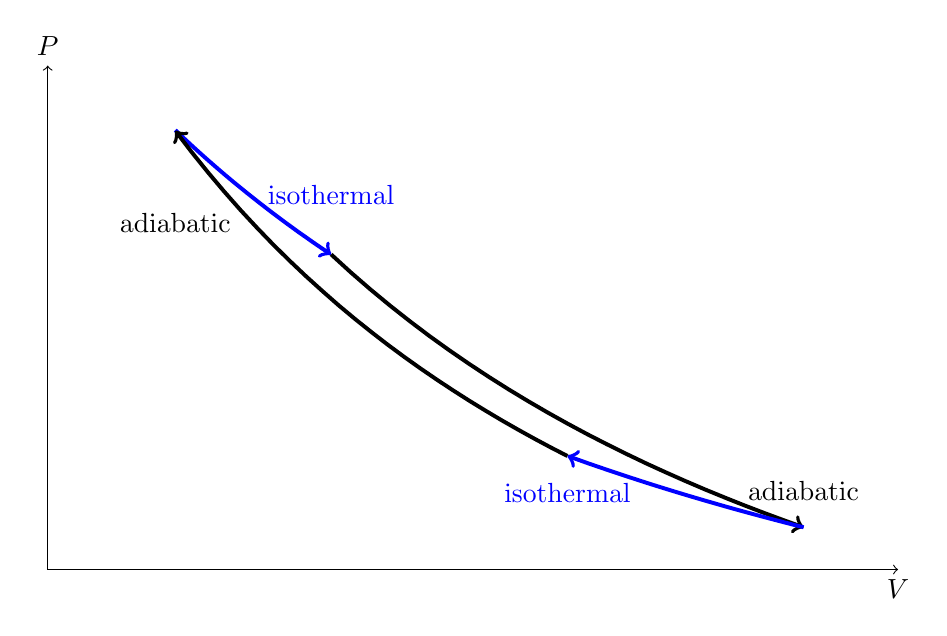
\begin{tikzpicture}[x=6cm, y=8cm]
\draw [->] (1.4, 0.5) -- (3.2, 0.5) node[below]{$V$};
\draw [->] (1.4, 0.5) -- (1.4, 1.3)  node[above]{$P$};
\draw [->, line width=0.05cm, blue, domain=1.67:2.0]  plot(\x, {  2.0/\x})           node[above, yshift=0.5cm] {isothermal};
\draw [->, line width=0.05cm, black,domain=2.00:3.0]  plot(\x, {2.639/((\x)^(1.4))}) node[above, yshift=0.2cm] {adiabatic};
\draw [->, line width=0.05cm, blue, domain=3.0:2.50]  plot(\x, {1.701/\x})           node[below, yshift=-0.2cm] {isothermal};
\draw [->, line width=0.05cm, black,domain=2.5:1.67]  plot(\x, {2.453/((\x)^(1.4))}) node[below, yshift=-0.9cm] {adiabatic};
\end{tikzpicture}
\caption{The Carnot cycle.}
\end{figure}

{\bf Exercises}\\
\begin{enumerate}
\item Why must you put an air conditioner in the window of a building, rather than in the middle of a room?
\item Can you cool off your kitchen by leaving the refrigerator door open?
\item Prove that the efficiency of a Carnot engine is 1-$\frac{T_c}{T_h}$
\end{enumerate}

\section{Homework}
Problem 4.2, 4.3, 4.11


